\begin{frame}
    \frametitle{Motores de Corriente Continúa (DC Motors)}
    \note{Información extraída de https://youtu.be/pEVsedl2KO4?si=_cwQpRPPUnQ04B3c}
    
    \begin{itemize}
        \item Dos imanes permanentementes estacionarios, que conforman los polos norte (azul) y sur (rojo).
        \item Electromagnetismo induce torque
        \item Los Anillos divididos + brushes cambian la dirección de la corriente
    \end{itemize}
    
    \note{La idea principal es que cuando hay una corriente que fluye a través del de un cable (bobina) y dicha bobina se encuentra en el centro de un campo magnético (generado por los imanes externos), dicha bobina va a experimentar una fuerza.}
    
    \note{En el eje del motor hay anillo dorado que funciona como cepillo para que circule corriente a través de la bobina (que se encuentra dentro de un campo magnético). Observar que el anillo tiene una ranura para solo permitir pasar corriente en la bobina cuando esta este ubicada de manera tal que la corriente circule de manera perpendicular al campo magnético generado por los imanes.}
    
    \note{Se conectan los cables positivo y negativo a una batería, haciendo que pase corriente a través de la bobina. Los imanes norte y sur generan un campo magnético horizontal y la corriente que circula a través de la bobina genera una campo eléctrico en una dirección perpendicular. Esto hace que se genera una fuerza en el eje, moviendolo 180 grados. De esta manera se convierte energía eléctrica en energía mecánica de rotación.}
    
    \begin{figure}[!h]
        \subfloat[]{
            \movie[autostart,poster,loop,showcontrols]{\includegraphics[width=0.2\columnwidth,valign=m]{images/dc_motor_3d_video.jpg}}{videos/dc_motor_3d.mp4}
        }
        \subfloat[]{
            \movie[autostart,poster,loop,showcontrols]{\includegraphics[width=0.2\columnwidth,valign=m]{images/dc_motor_video.jpg}}{videos/dc_motor.mp4}
        }
        \subfloat[]{
            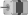
\includegraphics[width=0.3\columnwidth,valign=m]{images/dc_motor.pdf}
        }
    \end{figure}
    
\end{frame}

\begin{frame}
    \frametitle{Controladores de Motores DC}
    \note{Información extraída de https://youtu.be/pEVsedl2KO4?si=_cwQpRPPUnQ04B3c}
    
    \begin{itemize}
        \item Más corriente implica más rotación
        \item ¿Cómo modular corriente usando una señal digital?
        \item \emph{Pulse Width Modulation} (PWM)
        \item Duty cycle = ratio de tiempo vs periodo
    \end{itemize}
    
    \begin{figure}[!h]
        \subfloat[]{
            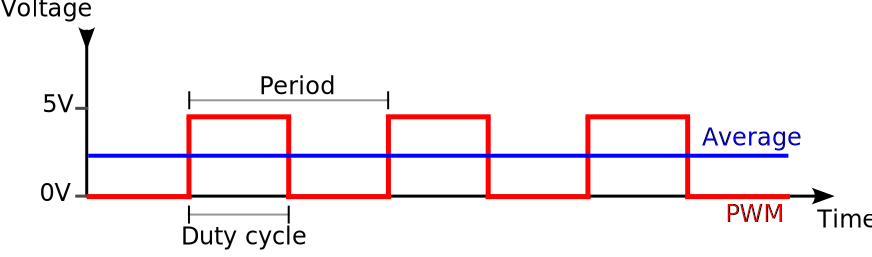
\includegraphics[width=0.6\columnwidth,valign=m]{images/pwm_signal.pdf}
        }
        \hfill
        \subfloat[]{
            \includegraphics[width=0.3\columnwidth,valign=m]{images/dc_motor_driver_2x15A_lite.jpg}
        }
    \end{figure}
    
    \note{Cuando el pulso está arriba significa que es máxima corriente y por lo tanto la máxima velocidad que el motor puede tener. Duty cycle es cuanto tiempo dura el pulso. Entonces, si queremos ir a 1/4 de la velocidad máxima del motor entonces el pulso solo durará 1/4 del tiempo.}
    
    \note{La placa de ejmplo contiene 4 chips controladores, permitiendo controlar 4 motores}
    
    
\end{frame}

\begin{frame}
    \frametitle{Open loop vs feedback control}
    \note{Información extraída de https://youtu.be/pEVsedl2KO4?si=_cwQpRPPUnQ04B3c}
    
    \note{En la práctica, los motores no son perfectos. No van a la velocidad exacta que les pedimos (tienen error).}
    
    \begin{figure}[!h]
        \subfloat[Open loop control]{
            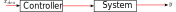
\includegraphics[width=0.6\columnwidth,valign=m]{images/open_loop_control.pdf}
        }
        
        \subfloat[Feedback control]{
            \includegraphics[width=0.7\columnwidth,valign=m]{images/feedback_control.pdf}
        }
    \end{figure}
    
    \note{en las figuras system hace referencia al motor.}
    
    \note{En Open Loop Control, e da un valor deseado de velocidad (por ejemplo: número de rotaciones por minuto), el controlador envía corriente al motor para cumplir dicha velocidad, el motor se mueve pero no sabemos a qué velocidad exactamente.}
    
    \note{En Feedback Control, se da un valor deseado de velocidad (por ejemplo: número de rotaciones por minuto), el controlador envía corriente al motor para cumplir dicha velocidad, el motor se mueve pero ahora podemos sensar a qué velocidad se está moviendo (por ejemplo con un encoder). Si hay una diferencia entra la velocidad deseada y la velocidad de salida, el controlador debería arreglar dicha diferencia.}
    
\end{frame}

\begin{frame}
    \frametitle{Ejemplo de Feedback control}
    \note{Información extraída de https://youtu.be/pEVsedl2KO4?si=_cwQpRPPUnQ04B3c}
    
    \begin{center}
        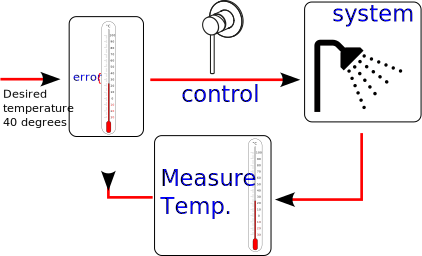
\includegraphics[width=0.6\columnwidth,valign=m]{images/temperature_feedback_control.pdf}
    \end{center}

    
\end{frame}

\begin{frame}
    \frametitle{Diagrama de bloques}
    \note{Información extraída de https://youtu.be/pEVsedl2KO4?si=_cwQpRPPUnQ04B3c}
    
    \begin{center}
        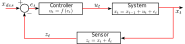
\includegraphics[width=0.8\columnwidth]{images/feedback_control_math.pdf}
    \end{center}
   
\end{frame}

\begin{frame}
    \frametitle{On-Off control}
    \note{Información extraída de https://youtu.be/pEVsedl2KO4?si=_cwQpRPPUnQ04B3c}
    
    \begin{center}
        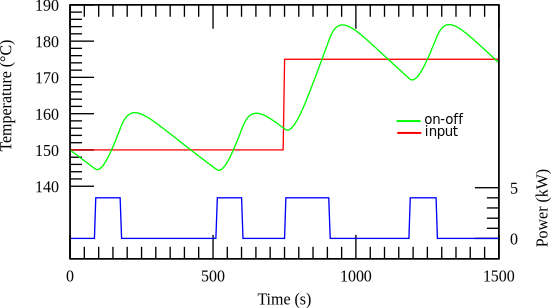
\includegraphics[width=0.8\columnwidth]{images/pid_control_on_off.pdf}
    \end{center}
    
    \note{Información extraída dehttps://www.zhinst.com/americas/de/resources/principles-of-pid-controllers}
    
    \note{Información extraída de https://newton.ex.ac.uk/teaching/CDHW/Feedback/ControlTypes.html}
    
\end{frame}

\begin{frame}
    \frametitle{Proportional control}
    \note{Información extraída de https://youtu.be/pEVsedl2KO4?si=_cwQpRPPUnQ04B3c}
    
    \begin{itemize}
        \item P-Control: $\controlCommand_{t} = K_{p} \error_{t}$ donde $\error_{t} = x_{des} - x_{t}$
    \end{itemize}
    
    \begin{center}
        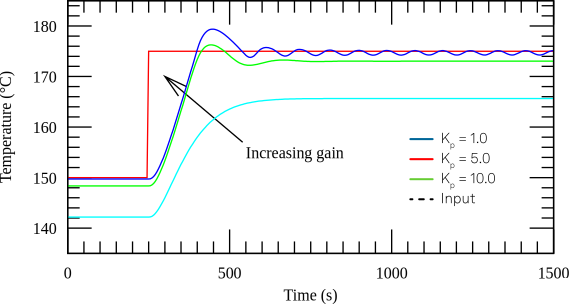
\includegraphics[width=0.8\columnwidth]{images/pid_control_proportional.pdf}
    \end{center}
    
    \note{Información extraída dehttps://www.zhinst.com/americas/de/resources/principles-of-pid-controllers}
    \note{Información extraída de https://newton.ex.ac.uk/teaching/CDHW/Feedback/ControlTypes.html}
    
\end{frame}

\begin{frame}
    \frametitle{Proportional+Derivative control}
    \note{Información extraída de https://youtu.be/pEVsedl2KO4?si=_cwQpRPPUnQ04B3c}
    
    \begin{itemize}
        \item PD-Control: $\controlCommand_{t} = K_{d} \error_{t}$
    \end{itemize}
    
    \begin{center}
        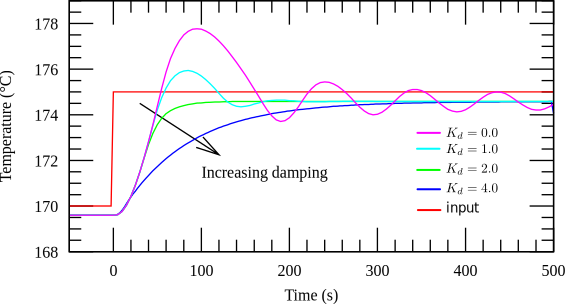
\includegraphics[width=0.8\columnwidth]{images/pid_control_derivative.pdf}
    \end{center}
    
    Un damping (amortiguación) demasiado pequeña produce overshoot y ringing, demasiado grande provoca una respuesta innecesariamente lenta.
    
    \note{Información extraída dehttps://www.zhinst.com/americas/de/resources/principles-of-pid-controllers}
    \note{Información extraída de https://newton.ex.ac.uk/teaching/CDHW/Feedback/ControlTypes.html}
    
    \note{Esta es la forma de control más sencilla y utilizada por casi todos los termostatos domésticos. Cuando el horno está más frío que la temperatura establecida, el calentador se enciende a la potencia máxima, M, y una vez que el horno está más caliente que la temperatura establecida, el calentador se apaga por completo. Las temperaturas de encendido y apagado se hacen deliberadamente para que difieran en una pequeña cantidad, conocida como histéresis H, para evitar que el ruido encienda el calentador rápidamente e innecesariamente cuando la temperatura está cerca del punto de ajuste. Las fluctuaciones de temperatura mostradas en el gráfico son significativamente mayores que la histéresis debido a la importante capacidad calorífica del elemento calefactor.}
\end{frame}

\begin{frame}
    \frametitle{Proportional+Integral+Derivative control}
    \note{Información extraída de https://youtu.be/pEVsedl2KO4?si=_cwQpRPPUnQ04B3c}
    
    \begin{itemize}
        \item PID-Control: $\controlCommand_{t} = K_{p} \error_{t}$
    \end{itemize}
    
    \begin{center}
        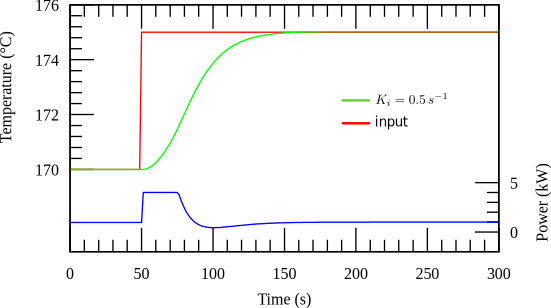
\includegraphics[width=0.8\columnwidth]{images/pid_control_integral.pdf}
    \end{center}
    
    \note{Información extraída dehttps://www.zhinst.com/americas/de/resources/principles-of-pid-controllers}
    \note{Información extraída de https://newton.ex.ac.uk/teaching/CDHW/Feedback/ControlTypes.html}
    
\end{frame}

\subsection{Position Control}

\begin{frame}
    \frametitle{Motivación: Position Control}
    \note{Información extraída de https://youtu.be/pEVsedl2KO4?si=_cwQpRPPUnQ04B3c}
    
    \begin{itemize}
        \item Mover el robot a una ubicación deseada $x_{des}$
        \item ¿Cómo generamos una señal de control adecuada $\controlCommand$?
        \item La localización del robot se estima mediante mediciones $\measurement$ de un sensor
    \end{itemize}
    
\end{frame}

\begin{frame}
    \frametitle{Cinemática de un cuerpo rígido}
    \note{Información extraída de https://youtu.be/pEVsedl2KO4?si=_cwQpRPPUnQ04B3c}
    
    \begin{itemize}
        \item Consideremos a un robot como un punto de masa
        \item Moviendo libremente en el espacio 1D
    \end{itemize}
    
\end{frame}

\begin{frame}
    \frametitle{Cinemática de un cuerpo rígido}
    \note{Información extraída de https://youtu.be/pEVsedl2KO4?si=_cwQpRPPUnQ04B3c}
    
    
    
    \TODO{Agregar imágenes }
    
\end{frame}


\begin{frame}
    \frametitle{P-control}
    \note{Información extraída de https://youtu.be/pEVsedl2KO4?si=_cwQpRPPUnQ04B3c}
    
    \begin{itemize}
        \item \TODO{Agregar imágenes }
    \end{itemize}
    
\end{frame}

\begin{frame}
    \frametitle{PD-control}
    \note{Información extraída de https://youtu.be/pEVsedl2KO4?si=_cwQpRPPUnQ04B3c}
    
    \begin{itemize}
        \item \TODO{Agregar imágenes }
    \end{itemize}
    
\end{frame}


\begin{frame}
\frametitle{PID-control}
\note{Información extraída de https://youtu.be/pEVsedl2KO4?si=_cwQpRPPUnQ04B3c}

\begin{itemize}
    \item \TODO{Agregar imágenes }
\end{itemize}

\end{frame}



\begin{frame}
    \frametitle{PID-control}
    \note{Información extraída de https://youtu.be/pEVsedl2KO4?si=_cwQpRPPUnQ04B3c}
    
    \begin{itemize}
        \item Estimar el error sistemático...
        \item PID-Control:
        \begin{equation*}
            \controlCommand_{t} = K_{p} \left(x_{des} - x_{t}\right) + K_{d} \left(\dot{x}_{des} - \dot{x}_{t} \right) + K_{i} \int_{0}^{t} \left( x_{des} - x_{t}\right) \, dt
        \end{equation*}
        
    \end{itemize}
    
    \begin{itemize}
        \item Funciona razonablemente para sistemas estables (con poco ruido)
        \item Puede ser peligroso en el caso en que se acumulen errores (\emph{wind-up effect})
    \end{itemize}
    
    \note{Si un robot se traba en un pozo y las ruedas siguen girando, la pose estimada por odometría y la verdadera localización del robot crece constantemente. El término integral del PID va a tomar valores enormes, ya que el error se acumula. En esta situación, si el robot se destrababa, vamos a tener una velocidad enorme y por lo tanto hacer que robot por ejemplo salte. Para esto el término integral puede únicamente tomar una ventana de tiempo (por ejemplo los últimos 5 segundos).}
    
    \note{El wind-up effect se refiere a cuando le damos un comando de control al robot pero los actuadores no son capaces de alcanzar el control solicitado. Esto puede ocasionar también que se acumule error.}
    
    
    \note{Información extraída dehttps://www.zhinst.com/americas/de/resources/principles-of-pid-controllers}
    \note{Información extraída de https://newton.ex.ac.uk/teaching/CDHW/Feedback/ControlTypes.html}
    
\end{frame}

\begin{frame}
    \frametitle{PID-control: Resumen}
    \note{Información extraída de https://youtu.be/pEVsedl2KO4?si=_cwQpRPPUnQ04B3c}
    
    \begin{itemize}
        \item P = control proportional, suficiente para la mayoría de los casos
        \item PD = reduce overshoot (por ejemplo, cuando la aceleración del vehículo puede ser controlada)
        \item PI = compensa errores o bias sistemáticos
        \item PID = combinación de todas las propiedades anteriores
    \end{itemize}
    
\end{frame}

\subsection{Trajectory control}

\begin{frame}
    \frametitle{Aplicación: Siguiendo una trayectoria}
    \note{Información extraída de https://youtu.be/pEVsedl2KO4?si=_cwQpRPPUnQ04B3c}
    
    \TODO{Agregar imagen}
    
\end{frame}

\begin{frame}
    \frametitle{Arquitectura de control}
    \note{Información extraída de https://youtu.be/pEVsedl2KO4?si=_cwQpRPPUnQ04B3c}
    
    \begin{center}
        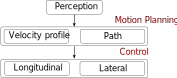
\includegraphics[width=0.8\columnwidth]{images/control_architecture2.pdf}
    \end{center}
    
     \note{Percepción: a través de los sensores armar un mapa del entorno}
     \note{Trayectoria = camino +perfil de velocidades. En cada pose del camino debemos saber con qué velocidad tenemos que llegar. Que cada punto de la trayectoria tenga un perfil de velocidad permite que el robot pueda moverse de manera suave de una pose a la otra.}
     \note{El control se divide en dos partes: longitudinal y lateral. El control Longitudinal hace referencia sobre la dirección de movimiento, es decir controlar la velocidad lineal. El control Lateral hace referencia que el robot este cerca del camino a seguir.}
\end{frame}

\begin{frame}
    \frametitle{Generación de trayectorias}
    \note{Información extraída de https://youtu.be/pEVsedl2KO4?si=_cwQpRPPUnQ04B3c}
    
    \begin{center}
        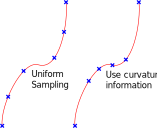
\includegraphics[width=0.6\columnwidth]{images/trajectory_generation.pdf}
    \end{center}
    
\end{frame}

\begin{frame}
    \frametitle{Ackermann Steering}
    \note{Información extraída de https://youtu.be/pEVsedl2KO4?si=_cwQpRPPUnQ04B3c}
    
    \begin{center}
        \includegraphics[width=0.6\columnwidth]{images/ackermann_steering.pdf}
    \end{center}
    
\end{frame}

\begin{frame}
    \frametitle{Ackermann Kinematics}
    \note{Información extraída de https://youtu.be/pEVsedl2KO4?si=_cwQpRPPUnQ04B3c}
    
    Estado: $\begin{bmatrix} x & y & \theta & \delta \end{bmatrix}^{\top}$ con $\delta = \tan^{-1}{\left(\frac{d}{r}\right)}$
    
    Control: $\begin{bmatrix} v & \dot{\delta} \end{bmatrix}^{\top}$
    
    
    \begin{center}
        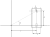
\includegraphics[width=0.6\columnwidth]{images/ackermann_kinematics.pdf}
    \end{center}
    
\end{frame}

\begin{frame}
    \frametitle{Control}
    \note{Información extraída de https://youtu.be/pEVsedl2KO4?si=_cwQpRPPUnQ04B3c}
    
    Restricciones:
    
    $v < v_{\max}$
    
    $v < |\delta_{\max}|$
    
    
    \begin{center}
        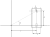
\includegraphics[width=0.6\columnwidth]{images/ackermann_kinematics.pdf}
    \end{center}
    
\end{frame}

\begin{frame}
    \frametitle{Longitudinal Control}
    \note{Información extraída de https://youtu.be/pEVsedl2KO4?si=_cwQpRPPUnQ04B3c}
        
    \begin{center}
        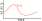
\includegraphics[width=0.6\columnwidth]{images/longitudinal_control.pdf}
    \end{center}
    
    \only<1->{¿Cómo podemos obtener esto?}
    \only<2->{Control PID}
    
\end{frame}


\begin{frame}
    \frametitle{Lateral Control}
    \note{Información extraída de https://youtu.be/pEVsedl2KO4?si=_cwQpRPPUnQ04B3c}
    
    \begin{center}
        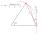
\includegraphics[width=0.6\columnwidth]{images/lateral_control.pdf}
    \end{center}

\end{frame}

\begin{frame}
    \frametitle{Control en cascada}
    \note{Información extraída de https://youtu.be/pEVsedl2KO4?si=_cwQpRPPUnQ04B3c}
    
    \begin{center}
        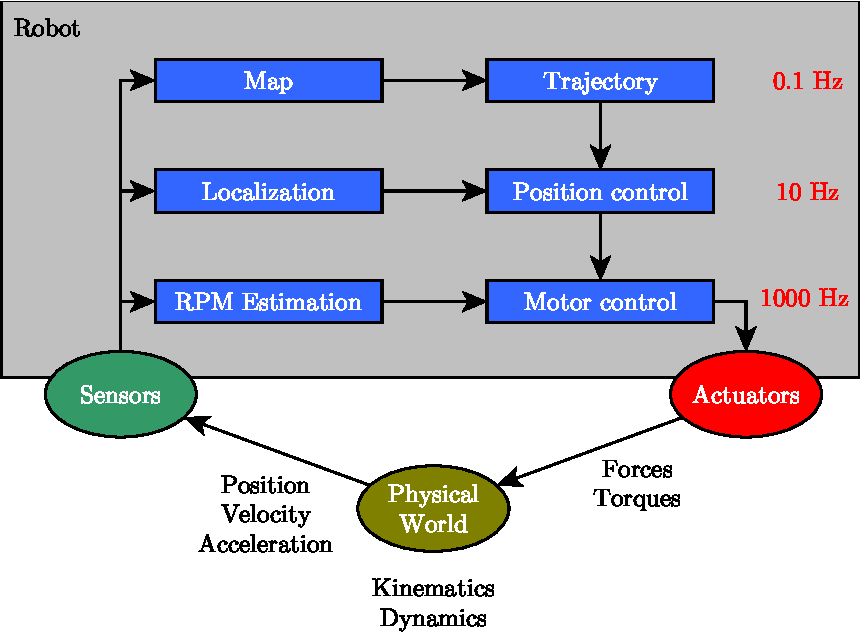
\includegraphics[width=0.7\columnwidth]{./images/control_architecture_phrequency.pdf}
    \end{center}
    
\end{frame}

\begin{frame}
    \frametitle{Objetivos del diseño de control}
    \note{Información extraída de https://youtu.be/pEVsedl2KO4?si=_cwQpRPPUnQ04B3c}
    
    \begin{itemize}
        \item Precisión
        \item Seguridad
        \item Robustez
        \item Tiempo de respuesta
        \item Mantenimiento
        \item y otros objetivos específicos de la aplicación...
    \end{itemize}
    
\end{frame}


\begin{frame}
    \frametitle{Técnicas de control avanzadas}
    \note{Información extraída de https://youtu.be/pEVsedl2KO4?si=_cwQpRPPUnQ04B3c}
    
    \begin{itemize}
        \item Optimal control
        \item Linear Quadratic Regulator (LQR)
        \item Robust control
        \item Adaptive control
        \item Failsafe control
        \item Learning based control
        \item Muchas más técnicas...
    \end{itemize}
    
\end{frame}

\begin{frame}
    \frametitle{Optimal Control}
    \note{Información extraída de https://youtu.be/pEVsedl2KO4?si=_cwQpRPPUnQ04B3c}
    
    \begin{itemize}
        \item Encontrar el controlador que de la mejor performance.
        \item ¿Cómo medir la performance?
        \item ¿Cuál sería una buena medida de performance?
        \begin{itemize}
            \item Minimizar el error?
            \item Minimizar los controles necesarios?
            \item Una combinación de ambas?
        \end{itemize}
    \end{itemize}
    
\end{frame}

\begin{frame}
    \frametitle{Linear Quadratic Regulator (LQR)}
    \note{Información extraída de https://youtu.be/pEVsedl2KO4?si=_cwQpRPPUnQ04B3c}
    
    \begin{itemize}
        \item Sistema \textbf{lineal} de tiempo discreto
            \begin{equation*}
                \state_{k+1} = A \state_{k} + B \controlCommand_{k}
            \end{equation*}
        \item Función de costo \textbf{cuadrática}
            \begin{equation*}
                \jacobian = \sum{\left(\state_{k}^{\top} Q \state_{k} + \controlCommand_{k}^{\top} R \controlCommand_{k}\right)}
            \end{equation*}
        \item \textbf{Objetivo}: Encontrar el control de menor costo.
    \end{itemize}
    
\end{frame}

\begin{frame}
    \frametitle{Control No-lineal}
    \note{Información extraída de https://youtu.be/pEVsedl2KO4?si=_cwQpRPPUnQ04B3c}
    
    \begin{itemize}
        \item ¿Qué si el sistema tiene dinámicas no-lineales?
        \item Resolver un problema de optimización no-lineal es costoso
        \item Linearizar el sistema y resolver como LQR
        \item Resolver el problema de optimización no-lineal para un un horizonte cercano
        \item Resulta en \emph{Model Predictive Controller} (MPC)
    \end{itemize}
    
\end{frame}

\begin{frame}
    \frametitle{Control Adaptativo}
    \note{Información extraída de https://youtu.be/pEVsedl2KO4?si=_cwQpRPPUnQ04B3c}
    
    \begin{itemize}
        \item \textbf{idea:} cambiar la ley de control por la estimarción de parámetros de sistema y actualizarlo en tiempo-real
        \item Adaptar coeficientes basados en meta-observaciones
        \item Lidiar con tiempo variable o incerteza de parámetros
        \item Ejemplo: Decrece en aviones como la masa decrece debido al consumo de combustible 
    \end{itemize}
    
\end{frame}

\begin{frame}
    \frametitle{Control Robustos}
    \note{Información extraída de https://youtu.be/pEVsedl2KO4?si=_cwQpRPPUnQ04B3c}
    
    \begin{itemize}
        \item \textbf{Idea:} Diseño que explícitamente considera la incertidumbre.
        \item Define una cota para la incertidumbre en modelo de parámetros.
        \item La ley de control garantiza estabilidad siempre y cuando la incertidumbre este entre las cotas.
        \item Pero la ley de control es \textbf{estática} a diferencia del control adaptativo.
    \end{itemize}
    
\end{frame}

\begin{frame}
    \frametitle{Control basado en aprendizaje}
    \note{Información extraída de https://youtu.be/pEVsedl2KO4?si=_cwQpRPPUnQ04B3c}
    
    \begin{center}
        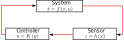
\includegraphics[width=0.7\columnwidth]{./images/learning_based_control.pdf}
    \end{center}
   
\end{frame}

\begin{frame}
    \frametitle{Resumen}
    \note{Información extraída de https://youtu.be/pEVsedl2KO4?si=_cwQpRPPUnQ04B3c}
    
    \begin{itemize}
        \item Motores y controles de bajo nivel
        \item Feedback control
        \item Control PID
        \item Control para seguimiento de caminos
        \item Algunas técnicas de control avanzadas
    \end{itemize}
    
\end{frame}




